% ================================
% ABV-IIITM Thesis Title Page
% Compile with: pdflatex
% ================================
\documentclass[12pt,a4paper]{report}

% --- Layout & graphics
\usepackage[a4paper,margin=1in]{geometry}
\usepackage{graphicx}
\usepackage{lmodern}
\usepackage[T1]{fontenc}
\usepackage[utf8]{inputenc}
\usepackage{setspace}
\usepackage{tabularx}
\usepackage{amsmath}
\usepackage{enumitem}
\usepackage{tikz}
% figures & subfigures
\usepackage{caption}
\usepackage{subcaption}   % <-- defines subfigure
\usepackage{placeins}     % optional:
\usepackage{caption}
\usepackage{subcaption}
\usepackage{placeins}
\usepackage{pdflscape} % for the landscape waveform page

% Tighter but clean float spacing + smaller captions
\captionsetup[figure]{font=small,labelfont=bf}
\captionsetup[sub]{font=small}
\setlength{\textfloatsep}{10pt plus 2pt minus 2pt}
\setlength{\floatsep}{10pt plus 2pt minus 2pt}
\setlength{\intextsep}{10pt plus 2pt minus 2pt}

\FloatBarrier

\usetikzlibrary{arrows.meta,positioning,shapes.geometric,shapes.misc,fit,automata}
\usepackage{booktabs}   % optional, for nicer tables

\usepackage[backend=biber,style=ieee,sorting=none,defernumbers=true]{biblatex}
\addbibresource{refs.bib}

\newcolumntype{L}{>{\raggedright\arraybackslash}X}


% --- Toggle logo on/off
\newif\ifuseLogo
\useLogotrue
\newcommand{\LogoPath}{Logo.jpg}

% --------- EDIT THESE FIELDS ---------
\newcommand{\ThesisTitle}{Design and Optimization of AES-256 Architecture
with Clock-Gating}
\newcommand{\Programme}{M.Tech.\ (\textit{ICD\&T})}
\newcommand{\Department}{Department of Electrical \& Electronics Engineering}
\newcommand{\AuthorName}{Paras Arya}
\newcommand{\RollNo}{2024ICD-006}
\newcommand{\Supervisor}{Dr.\ Alok Kumar Kamal}
% \newcommand{\ExternalSupervisor}{Revanth Thimmappa}
% \newcommand{\ExternalSupervisorDesignation}{Senior Software Engineer at Rakuten India}
\newcommand{\InstituteName}{ABV--Indian Institute of Information Technology \& Management, Gwalior}
\newcommand{\InstituteCity}{Gwalior, India}
\newcommand{\SessionDates}{December~10, 2025}
% -------------------------------------

% QoL
\usepackage{microtype}
\usepackage{csquotes}

% Bibliography
\usepackage[backend=biber,style=ieee,sorting=none]{biblatex}
\addbibresource{refs.bib}

% Hyperlinks
\usepackage[hidelinks]{hyperref}
\hypersetup{
  pdftitle   = {Accelerating the Development Lifecycle through Mock-Server-Based Integration Testing of Systems Under Test},
  pdfauthor  = {Paras Arya},
  pdfsubject = {M.Tech Report},
  pdfcreator = {LaTeX}
}

% No page number on title page
\pagestyle{empty}

\begin{document}

% ---------- TITLE PAGE ----------
\begin{titlepage}
  \centering
  {\LARGE\bfseries \ThesisTitle \par}
  \vspace{1.2cm}

  {\large A report submitted in \textit{partial fulfilment} of the requirements\\
  for the award of the degree of\\[0.6ex]
  \textbf{Master of Technology (\Programme)}\par}
  \vspace{1.2cm}

  {\large \textbf{by}}\par
  \vspace{0.35cm}
  {\Large \textbf{\AuthorName}}\par
  \vspace{0.15cm}
  {\large Roll No.\ \textbf{\RollNo}}\par
  \vspace{1.2cm}

  {\large \textbf{Under the supervision of}}\par
  \vspace{0.35cm}
  {\large \textbf{\Supervisor}}\par
  % {\large \textbf{and}}\\[0.2cm]
  % {\large \textbf{\ExternalSupervisor}}\par
  % {\scriptsize \textit{\ExternalSupervisorDesignation}}\par
  \vspace{1.2cm}

  {\large \Department}\par
  \vspace{0.4cm}

  \ifuseLogo
    \includegraphics[width=2.5cm]{\LogoPath}\par
    \vspace{0.6cm}
  \fi

  {\large \InstituteName}\par
  \vspace{0.2cm}
  {\large \InstituteCity}\par
  \vspace{0.8cm}

  {\large \SessionDates}\par

  \vfill
\end{titlepage}

% ---------- FRONT MATTER (roman) ----------
\pagenumbering{roman}
\pagestyle{plain}

% --- Declaration ---
\cleardoublepage
\addcontentsline{toc}{section}{Declaration}   % article -> section
\thispagestyle{empty}
\begin{center}
  {\Large \textbf{DECLARATION}}
\end{center}
\vspace{0.8cm}

I, \textbf{\AuthorName} (Roll No.\ \textbf{\RollNo}), hereby declare that the work presented
in the report entitled \textbf{``\ThesisTitle''}, submitted in partial fulfilment of the
requirements for the award of the degree of \textbf{Master of Technology (\Programme)} to
\textbf{\InstituteName}, is an authentic record of my own work carried out during
\textbf{\SessionDates} under the supervision of \textbf{\Supervisor} in the \textbf{\Department}.

\vspace{0.6cm}
This report has not been submitted for the award of any other degree or diploma of this or any
other institute. All sources of information used in the report—texts, figures, tables, and data—
have been duly acknowledged and cited.

\vspace{1.2cm}
\noindent
\begin{minipage}[t]{0.48\textwidth}
  \textbf{Date:} \rule{5cm}{0.4pt}\\[0.6cm]
  \textbf{Place:} \rule{4.8cm}{0.4pt}
\end{minipage}\hfill
\begin{minipage}[t]{0.48\textwidth}
  \raggedleft
  \textbf{Signature of the Candidate}\\[0.6cm]
  \rule{6cm}{0.4pt}\\[-0.1cm]
  \textbf{\AuthorName}\\
  Roll No.: \textbf{\RollNo}\\
  Programme: \Programme
\end{minipage}

\vspace{1.6cm}
\noindent
This is to certify that the above declaration by the candidate is correct to the best of my knowledge.

\vspace{1.2cm}
\noindent
\begin{minipage}[t]{0.48\textwidth}
  \textbf{Date:} \rule{5cm}{0.4pt}\\[0.6cm]
  \textbf{Place:} \rule{4.8cm}{0.4pt}
\end{minipage}\hfill
\begin{minipage}[t]{0.48\textwidth}
  \raggedleft
  \textbf{Signature of the Supervisor}\\[0.6cm]
  \rule{6cm}{0.4pt}\\[-0.1cm]
  \textbf{\Supervisor}
\end{minipage}

% --- Acknowledgements (airy) ---
\cleardoublepage
\addcontentsline{toc}{section}{Acknowledgements}
\thispagestyle{empty}
\begin{center}
  {\Large \textbf{ACKNOWLEDGEMENTS}}
\end{center}
\vspace{0.9cm}

\begin{center}
\begin{minipage}{0.92\textwidth}
\begin{spacing}{1.2}
{\large
I express my deepest gratitude to my supervisor, \textbf{\Supervisor}, for
his patient guidance, insightful discussions, and continuous encouragement
throughout the course of this work. His clarity of thought and emphasis on
first principles shaped both the problem formulation and the execution of this
report. I am grateful to the faculty and staff of the \textbf{\Department} at
\textbf{\InstituteName} for creating a supportive academic environment and for their timely help with laboratory facilities, software access, and logistics. I also thank the postgraduate office and administrative staff for their kind assistance with official procedures. My sincere thanks to my peers and labmates for the many helpful conversations, code reviews, and constructive feedback that improved the methodology and experiments presented here. Above all, I am profoundly thankful to my family and friends for their unwavering support, patience, and motivation during the preparation of this
report.
}
\end{spacing}
\end{minipage}
\end{center}

\vspace{1.8cm}
\noindent
\begin{minipage}[t]{0.48\textwidth}
  \textbf{Date:} \rule{5cm}{0.4pt}\\[0.6cm]
  \textbf{Place:} \InstituteCity
\end{minipage}\hfill
\begin{minipage}[t]{0.48\textwidth}
  \raggedleft
  \textbf{\AuthorName}\\
  Roll No.: \textbf{\RollNo}
\end{minipage}

% --- Abstract (compact, airy) ---
\cleardoublepage
\addcontentsline{toc}{section}{Abstract}
\thispagestyle{empty}
\begin{center}
  {\Large \textbf{ABSTRACT}}
\end{center}
\vspace{0.6cm}

\begin{center}
\begin{minipage}{0.92\textwidth}
\begin{spacing}{1.2}
{\large
\section*{Abstract}

This work presents the design, implementation, and optimization of AES 256 cryptographic architectures. The project begins by developing fully functional conventional AES encryption and decryption cores and validating them against standardized test vectors to ensure correctness for all key sizes. Building upon this foundation, an optimized architecture from prior research is studied and implemented. This architecture employs shared S Box hardware, conditional MixColumns bypassing, and a word serial datapath that together reduce area and computational redundancy.

To further improve energy efficiency, a clock gated low power extension is proposed. The method focuses on reducing switching activity in power intensive components including SubBytes, MixColumns, and the KeySchedule unit. Fine grained clock enables are used to deactivate unused logic without altering functional behavior. Insights from recent literature show that such gating strategies can reduce dynamic power while maintaining throughput.

The combined architecture provides a resource efficient and scalable solution for hardware based cryptographic acceleration. The contributions of this work include a complete and verified AES 128, AES 192, and AES 256 implementation, an optimized architecture with reduced area cost, and a clock gated extension aimed at lowering dynamic power. These results support the development of secure and energy efficient AES systems for VLSI and embedded applications.

}
\end{spacing}
\end{minipage}
\end{center}

\vspace{0.8cm}
\noindent\textbf{Keywords} AES architecture; clock gating; low power design; SubBytes; MixColumns; KeySchedule;

% \clearpage
% \section*{Abbreviations}\addcontentsline{toc}{section}{Abbreviations}

% \begin{center}
% \begin{minipage}{0.92\textwidth}
% \begin{spacing}{1.15}
% \begin{tabularx}{\textwidth}{@{}lL@{}}
% \textbf{AMS} & Account Management System \\
% \textbf{API} & Application Programming Interface \\
% \textbf{CI/CD} & Continuous Integration / Continuous Deployment \\
% \textbf{HTTP} & Hypertext Transfer Protocol \\
% \textbf{JSON} & JavaScript Object Notation \\
% \textbf{REST} & Representational State Transfer \\
% \textbf{SUT} & System Under Test \\
% \textbf{JAR} & Java ARchive \\
% \textbf{JUnit} & Java Unit Testing Framework \\
% \textbf{IDE} & Integrated Development Environment \\
% \textbf{UI} & User Interface \\
% \textbf{RMS} & Rakuten Management Services (contextual) \\
% \textbf{KYC} & Know Your Customer \\
% \textbf{PoC} & Proof of Concept \\
% \textbf{VM} & Virtual Machine \\
% \textbf{QA} & Quality Assurance \\
% \textbf{YAML} & Yet Another Markup Language \\
% \textbf{URL} & Uniform Resource Locator \\
% \textbf{CI} & Continuous Integration \\
% \textbf{CD} & Continuous Deployment \\
% \textbf{API Mock} & Simulated API endpoint for testing \\

% \end{tabularx}
% \end{spacing}
% \end{minipage}
% \end{center}


% --- TOC and Lists ---
\cleardoublepage
\tableofcontents
\cleardoublepage
\listoffigures
\cleardoublepage
% \listoftables

% ---------- MAIN MATTER (arabic) ----------
\cleardoublepage
\pagenumbering{arabic}

% (Your chapters/sections start here)
% ================================
% Chapter 1 — Introduction & Motivation (2–page target)
% Paste after you switch to \pagenumbering{arabic}
% ================================
% ==========================================================
\chapter{Introduction \& Motivation}

\section{Introduction}
The Advanced Encryption Standard (AES) remains the most widely adopted block cipher in
modern secure systems, supporting key lengths of 128, 192, and 256 bits. Its suitability for
hardware stems from a regular round-based structure, enabling efficient implementation on
FPGA and ASIC platforms. A variety of baseline AES architectures have been developed on
reconfigurable hardware, demonstrating functional correctness and area–throughput tradeoffs
\cite{sai_srinivas_fpga_2016, abhijith_high_2013}. Work on compact lookup-table based
transformations further reduced redundant hardware in S-Box and inverse S-Box circuits
\cite{rajeswara_rao_fpga_2017}. Systematic FPGA benchmarking environments such as
\cite{guruprasad2018evaluation} have contributed to consistent evaluation of AES hardware
cores across platforms.

Despite the algorithm's structural simplicity, conventional AES designs incur considerable
area and dynamic power due to duplicated round logic, continuous toggling of SubBytes and
MixColumns units, and the overhead of key schedule expansion. Optimized architectures have
attempted to address these issues through resource sharing and datapath restructuring.
Notably, the Virtex-7 optimized AES-256 design reported in 
\cite{gunasekaran_aes256_virtex7} introduced a unified S-Box/Inv-S-Box structure, a
word-serial datapath, and a combined MixColumns--AddRoundKey unit, achieving significant
reductions in hardware footprint. Such improvements align with early efforts to minimize
resource usage in high-performance FPGA realizations of AES
\cite{abhijith_high_2013, rajeswara_rao_fpga_2017}.

In recent years, power efficiency has emerged as a key design objective due to the growing
presence of AES engines in mobile, IoT, and battery-constrained environments. Studies such
as \cite{feng2021_energy_efficient_aes, ibrahim2021_highspeed_resourceefficient_aes}
demonstrate that even optimized datapaths can remain power-intensive when active every
cycle. As a result, selective activation techniques—primarily clock gating—have gained
traction. Fine-grained asynchronous activation methods proposed in
\cite{selvapriya2023lowpower} exhibit substantial savings by enabling only the logic
required in a given cycle. Similarly, gated-datapath approaches in 
\cite{darwish2022configurable} target MixColumns and SubBytes units to reduce unnecessary 
switching. Multi-domain gating strategies reported in \cite{lee2021multidomain} further 
demonstrate that isolating clock domains for S-Box, MixColumns, and KeySchedule blocks can 
achieve meaningful power reduction.

Direct application of clock gating to AES functional blocks has also been validated through 
FPGA experiments. In \cite{chodorowski2021_clockgated_aes}, simple gating of non-active
cycles led to measurable savings in switching power, while pipelined AES designs using
clock gating on 28 nm technology achieved notable improvements in energy per operation
\cite{prasanth2021_lowpower_aes_clockgating}. Additional S-Box-centric gating mechanisms 
have been explored in \cite{subramanian2021_adaptive_clockgated_sbox}, highlighting the 
benefits of turning off composite-field logic when unused.

Motivated by these developments, this thesis constructs a fully functional baseline AES
implementation supporting all three key sizes. The primary contribution is a systematic,
dual-architecture study: a \textbf{full-pipeline AES implementation} and a \textbf{finite
state machine (FSM) AES implementation} are both developed, characterized at baseline, and
subjected to two optimization phases. Phase~1 replaces GF multiplication using EXP3 and LN3
log-table lookups with \textit{xtime} arithmetic~\cite{wolkerstorfer_xtime_2002}, eliminating
512 table entries from every MixColumns instance across both architectures. Phase~2 introduces
clock enable guards on FSM state registers to suppress unnecessary switching when the datapath
is idle. The Virtex-7 AES-256 architecture of \cite{gunasekaran_aes256_virtex7} provides
structural context for the unified S-Box and combined MixColumns--AddRoundKey design choices
adopted in the FSM datapath. The pipeline implementation follows the parallel datapath
approach established in prior work~\cite{good_pipelined_aes_2005}, enabling high throughput
through unrolled round logic.


\section{Motivation}

Modern VLSI and FPGA systems place strict constraints on power consumption, silicon area, and resource utilization. Cryptographic accelerators such as AES are now integrated into a wide range of platforms including communication modules, embedded processors, cloud servers, and edge devices. These systems require secure and high throughput encryption while also maintaining low energy consumption and minimal hardware cost. Conventional AES architectures, although functionally correct, often rely on duplicated S Box hardware, full width datapaths, and continuously active functional units. This leads to considerable dynamic power usage and limits the practicality of deployment in energy constrained systems.

The increasing use of AES 256 further amplifies these challenges due to its larger number of rounds and the additional complexity of the KeySchedule unit. This results in higher switching activity, increased latency, and greater pressure on available FPGA resources. Therefore, there is a strong need for an AES architecture that reduces redundant computation, improves hardware reuse, and manages switching activity intelligently.

Recent research demonstrates that clock gating is one of the most effective techniques for reducing dynamic power in cryptographic hardware. Fine grained gating, as explored in \cite{selvapriya2023lowpower}, selectively activates functional units only when required. Gated datapath techniques reported in \cite{darwish2022configurable} show that disabling MixColumns and SubBytes during idle cycles can produce substantial power savings. Multi domain gating methods in \cite{lee2021multidomain} further validate the potential for controlling switching activity across independent AES components. These works highlight a clear opportunity to improve AES efficiency by combining structural optimizations with targeted power aware design.

In addition, the evaluation framework proposed in \cite{guruprasad2018evaluation} emphasizes the importance of systematic performance analysis for cryptographic hardware. While this framework does not focus on power minimization, it underscores the need for reproducible and structured comparison of architectural choices. Motivated by these insights, this work aims to design an AES architecture that is both area efficient and energy aware. By integrating hardware reuse techniques inspired by \cite{gunasekaran_aes256_virtex7} with selective clock gating strategies from recent low power research, the goal is to develop a scalable AES core that is optimized for modern FPGA and VLSI platforms.

A central goal is to quantify the area and power tradeoff between the two architectural
paradigms: the pipeline architecture~\cite{good_pipelined_aes_2005}, which provides high
throughput through full round unrolling, and the FSM
architecture~\cite{mcloone_fsm_aes_2003}, which achieves area efficiency through round
hardware reuse. The two optimization phases applied equally to both architectures provide a
controlled, reproducible comparison of these design tradeoffs.


\input{chapters/ch2}
\chapter{Background Work}

% -----------------------------------------------------
\section{Conventional AES Architecture}
% -----------------------------------------------------

AES consists of multiple rounds that process a one hundred twenty eight bit state matrix using
a sequence of transformations. The number of rounds depends on the key size: ten for AES
one hundred twenty eight, twelve for AES one hundred ninety two, and fourteen for AES
two hundred fifty six.

\begin{figure}[!htbp]
    \centering
    \includegraphics[width=0.85\linewidth]{figs/aes-image.png}
    \caption{Conventional AES encryption and decryption round structure.}
    \label{fig:aes_conventional}
\end{figure}

The encryption process begins with an initial AddRoundKey operation followed by repeated
rounds that apply SubBytes, ShiftRows, MixColumns, and AddRoundKey. In the final round,
MixColumns is omitted. The decryption flow applies the inverse operations in reverse order.
Although the functional structure is symmetric, the conventional hardware realization requires
separate S Box and inverse S Box units, along with distinct MixColumns and InvMixColumns
modules. This leads to high area consumption and continuous switching activity across large
combinational blocks.

To summarize, conventional AES hardware commonly includes:
\begin{itemize}
    \item sixteen S Box units for SubBytes
    \item sixteen inverse S Box units for InvSubBytes
    \item four MixColumns units and four InvMixColumns units
\end{itemize}

which results in increased area and dynamic power.

% -----------------------------------------------------
\section{Proposed Architecture in the Virtex Seven Implementation}
% -----------------------------------------------------

The Virtex seven optimized AES architecture \cite{gunasekaran_aes256_virtex7} introduces two major improvements:
\begin{enumerate}
    \item a unified S Box and inverse S Box structure
    \item a combined MixColumns and AddRoundKey unit
\end{enumerate}
along with a word serial datapath that reduces the number of parallel functional units.

% --------------------------
\subsection{Unified S Box and Inverse S Box}
% --------------------------

The key observation is that both SubBytes and InvSubBytes share the same multiplicative
inverse computation, differing only in the affine transformations before and after the inverse.

\begin{figure}[!htbp]
    \centering
    \includegraphics[width=0.85\linewidth]{figs/s-box.png}
    \caption{Unified S Box and inverse S Box structure.}
    \label{fig:unified_sbox}
\end{figure}

\begin{itemize}
    \item The multiplicative inverse computation is shared between SubBytes and InvSubBytes.
    \item A mode-select multiplexer chooses between the forward and inverse affine transforms.
\end{itemize}

This unified structure eliminates duplication and reduces the number of S Box units
significantly in both parallel and serialized datapaths.

% --------------------------
\subsection{Combined MixColumns and AddRoundKey Unit}
% --------------------------

MixColumns is not required in the initial round or the final round. The optimized design merges
MixColumns and AddRoundKey into a single configurable unit that bypasses MixColumns
when the round counter indicates round zero or the last round \cite{gunasekaran_aes256_virtex7}.

\begin{figure}[!htbp]
    \centering
    \includegraphics[width=0.85\linewidth]{figs/mix-col.png}
    \caption{Combined MixColumns and AddRoundKey datapath.}
    \label{fig:mix_combined}
\end{figure}

This conditional structure:
\begin{itemize}
    \item avoids unnecessary MixColumns computation,
    \item reduces switching activity in the MixColumns module,
    \item simplifies the data path, and
    \item enables hardware reuse across rounds.
\end{itemize}

% -----------------------------------------------------
\section{Word Serial Datapath and Scheduling}
% -----------------------------------------------------

The conventional AES state matrix contains sixteen bytes arranged as a four by four grid.
Parallel architectures therefore require sixteen S Boxes and four MixColumns units. The
optimized design processes one column at a time, reducing the required functional units.

\begin{figure}[!htbp]
    \centering
    \includegraphics[width=0.45\linewidth]{figs/state_parallel.png}
    \caption{Parallel processing structure requiring sixteen S Boxes and four MixColumns units.}
    \label{fig:state_parallel}
\end{figure}

\begin{figure}[!htbp]
    \centering
    \includegraphics[width=0.45\linewidth]{figs/state_serial.png}
    \caption{Word serial processing structure requiring four S Boxes and one MixColumns unit.}
    \label{fig:state_serial}
\end{figure}

A word serial schedule processes each column in multiple cycles. An example cycle schedule
for fourteen round AES two hundred fifty six is shown below.

\begin{figure}[!htbp]
    \centering
    \includegraphics[width=0.9\linewidth]{figs/schedule_round.png}
    \caption{Example operation schedule for a word serial AES datapath.}
    \label{fig:schedule}
\end{figure}

This approach preserves correctness while reducing hardware cost and switching activity.

% -----------------------------------------------------
\section{Pipeline Architecture}
% -----------------------------------------------------

The full pipeline AES architecture implements each round as a distinct combinational stage,
enabling new plaintext to be accepted every clock cycle once the pipeline is filled.
This parallelism maximizes throughput at the expense of area: all round stages are active
simultaneously, requiring the full set of SubBytes, ShiftRows, MixColumns, and AddRoundKey
units for every pipeline stage. For AES-128 with ten rounds this results in ten independent
copies of the round logic instantiated in hardware.

In the baseline implementation, MixColumns is realized using a GF(2\textsuperscript{8})
multiplier built on EXP3 and LN3 log tables (\texttt{aes\_mcol.sv}). Each table contains
256 entries, so the combined EXP3 and LN3 lookup contributes 512 table entries to the
datapath. Because every pipeline stage contains a MixColumns unit, these tables are
replicated across all round stages, resulting in the 38,766 LUT baseline observed during
Vivado synthesis for AES-128.

The pipeline architecture is used as a high-area reference in this work. Phase~1 replaces
the log-table GF multiplier with \textit{xtime} arithmetic, eliminating the 512-entry table
from every MixColumns instance and projecting a reduction to approximately 25,000--30,000
LUTs.

% -----------------------------------------------------
\section{FSM Architecture}
% -----------------------------------------------------

The FSM based AES architecture serializes the encryption and decryption datapath across
clock cycles using an explicit state machine. A single set of round hardware is shared across
all AES rounds by cycling through states: \texttt{IDLE}, \texttt{LOAD\_KEY},
\texttt{KEY\_EXPANSION}, \texttt{ENCRYPT\_ROUND} (repeated for each round), and
\texttt{FINAL\_ROUND}. Because the same hardware block processes all rounds sequentially,
the area footprint is substantially smaller than the pipeline architecture. The AES-128
FSM baseline measures 6,794 LUTs and 412 flip-flops.

% Requires in main.tex preamble: \usepackage{tikz}
% \usetikzlibrary{automata,positioning,arrows.meta}
\begin{figure}[!htbp]
\centering
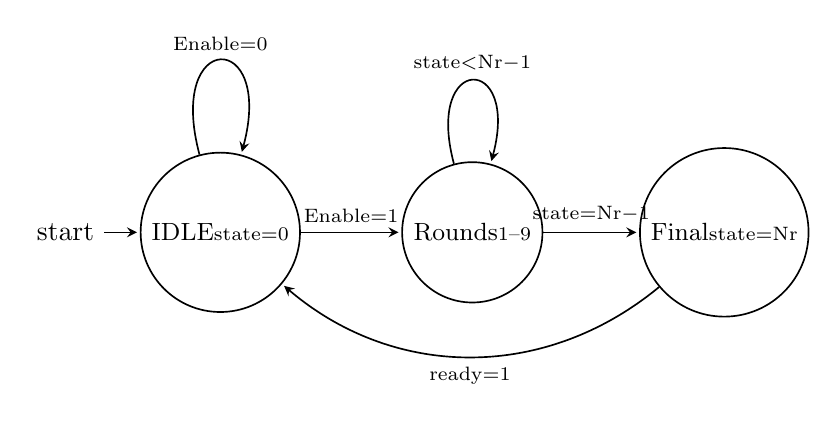
\begin{tikzpicture}[
    ->,>=stealth,
    shorten >=1pt,
    auto,
    node distance=3.2cm,
    semithick,
    every state/.style={draw, circle, minimum size=1.5cm, font=\small}
]

% States
\node[state, initial]           (IDLE)  {IDLE\\{\scriptsize state=0}};
\node[state, right of=IDLE]     (MID)   {Rounds\\{\scriptsize 1--9}};
\node[state, right of=MID]      (FINAL) {Final\\{\scriptsize state=Nr}};

% Transitions
\path (IDLE)  edge [loop above]  node {\scriptsize Enable=0}       (IDLE)
      (IDLE)  edge               node {\scriptsize Enable=1}        (MID)
      (MID)   edge [loop above]  node {\scriptsize state$<$Nr$-$1}  (MID)
      (MID)   edge               node {\scriptsize state=Nr$-$1}    (FINAL)
      (FINAL) edge [bend left=40] node {\scriptsize ready=1}        (IDLE);

\end{tikzpicture}
\caption{Encrypt FSM state diagram (AES-128, Nr=10). The CE guard
\texttt{r.state\,$\neq$\,0\,$\|$\,r.ready\,=\,1\,$\|$\,Enable\,=\,1}
freezes the packed state register when the FSM is idle, suppressing unnecessary
switching across all struct fields (Phase~2 optimization).}
\label{fig:encrypt_fsm}
\end{figure}

Three independent FSMs control the design: the encrypt FSM, the decrypt FSM, and the key
expansion FSM~\cite{mcloone_fsm_aes_2003}. Each FSM holds its computation state in a packed
register struct, enabling fine-grained clock enable gating in Phase~2.

Phase~2 of this work introduces clock enable (CE) guards on the FSM state registers. The
cipher and inverse cipher FSMs use the condition
\texttt{r.state != 0 || Enable == 1 || r.ready == 1} to gate register updates, ensuring
that the packed struct is frozen when the FSM is idle, preventing spurious switching on all
fields of the struct. The key expansion FSM uses a narrower guard
\texttt{r.state != 0 || Enable == 1} because the key expansion register has no ready bit
and does not require the ready-clear cycle present in the cipher FSMs. These CE guards
reduce dynamic switching power without altering functional behavior.

% -----------------------------------------------------
\section{Summary}
% -----------------------------------------------------

The Virtex-7 optimized AES architecture achieves substantial reduction in area and dynamic
power through structural reuse: a unified S-Box, a combined MixColumns--AddRoundKey unit, and
a word-serial datapath~\cite{gunasekaran_aes256_virtex7}.

The present work applies these principles within two distinct architectures:

\begin{itemize}
    \item \textbf{Pipeline architecture}~\cite{good_pipelined_aes_2005}: each AES round is
    instantiated as a separate combinational stage, enabling one new plaintext per clock cycle
    at the cost of replicating all round logic. Baseline AES-128 cost: 38,766 LUTs.

    \item \textbf{FSM architecture}~\cite{mcloone_fsm_aes_2003}: a single round hardware block
    is shared across all rounds under explicit state machine control. Baseline AES-128 cost:
    6,794 LUTs --- an 82\% area reduction relative to the pipeline.
\end{itemize}

Two optimization phases are applied to both architectures: Phase~1 replaces the EXP3/LN3
log-table GF multiplier with \textit{xtime} arithmetic~\cite{wolkerstorfer_xtime_2002},
targeting elimination of 512 table entries from each MixColumns instance. Phase~2 introduces
clock enable guards on the FSM state registers to reduce dynamic switching power when the
datapath is idle.
\input{chapters/ch4}
% =========================================
% Chapter X — Methodology
% =========================================
\chapter{Methodology}

\section{Overview}

The methodology adopted in this thesis follows a structured three stage workflow for 
designing and evaluating AES architectures of increasing optimization complexity. The 
workflow begins with the development of a conventional AES design, progresses to an 
architecturally optimized implementation based on reference literature, and concludes with 
a power aware extension achieved through clock gating. Each stage is followed by validation 
and comparative analysis to ensure correctness and measurable improvement.

\section{Methodology Flow}

\begin{figure}[!htpb]
\centering

% ---------- LEFT SIDE (PART 1) ----------
\begin{minipage}[t]{0.48\textwidth}
\centering
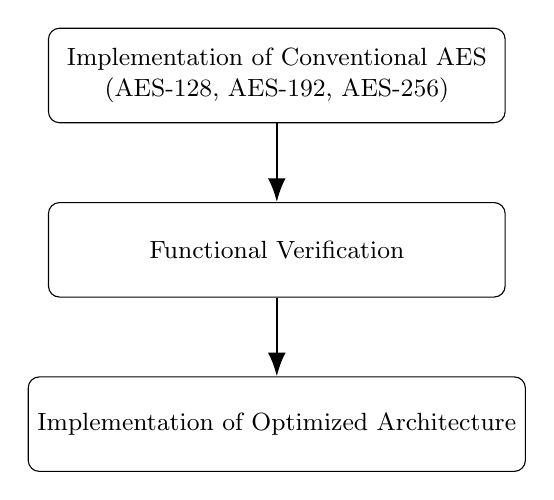
\begin{tikzpicture}[
    node distance = 1.0cm,
    every node/.style = {font=\small},
    box/.style = {
        rectangle,
        rounded corners,
        draw,
        align=center,
        minimum width=5.8cm,
        minimum height=1.2cm
    },
    arrow/.style = {
        -{Latex[length=3mm]},
        thick
    }
]

\node[box] (step1) {Implementation of Conventional AES \\ (AES-128, AES-192, AES-256)};
\node[box, below=of step1] (verify1) {Functional Verification};
\node[box, below=of verify1] (step2) {Implementation of Optimized Architecture};

\draw[arrow] (step1) -- (verify1);
\draw[arrow] (verify1) -- (step2);

\end{tikzpicture}
\caption*{Baseline AES and Optimized Architecture}
\end{minipage}
\hfill
% ---------- RIGHT SIDE (PART 2) ----------
\begin{minipage}[t]{0.48\textwidth}
\centering
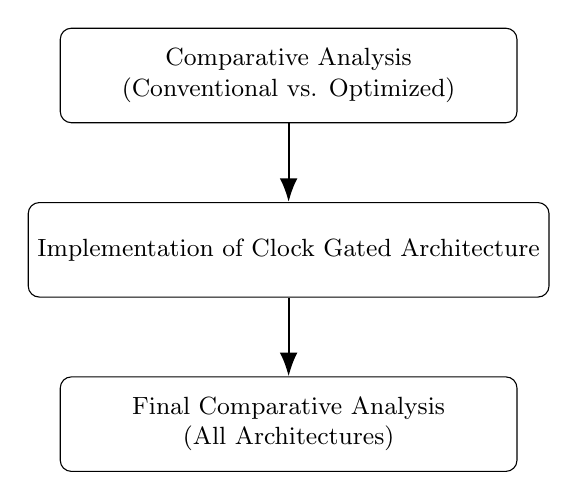
\begin{tikzpicture}[
    node distance = 1.0cm,
    every node/.style = {font=\small},
    box/.style = {
        rectangle,
        rounded corners,
        draw,
        align=center,
        minimum width=5.8cm,
        minimum height=1.2cm
    },
    arrow/.style = {
        -{Latex[length=3mm]},
        thick
    }
]

\node[box] (compare1) {Comparative Analysis \\ (Conventional vs. Optimized)};
\node[box, below=of compare1] (step3) {Implementation of Clock Gated Architecture};
\node[box, below=of step3] (compare2) {Final Comparative Analysis \\ (All Architectures)};

\draw[arrow] (compare1) -- (step3);
\draw[arrow] (step3) -- (compare2);

\end{tikzpicture}
\caption*{Clock Gating and Final Comparison}
\end{minipage}

\caption{Side-by-side methodology flowcharts for AES architecture design}
\label{fig:methodology_flow_sidebyside}

\end{figure}


\section{Extended Methodology for Pipeline and FSM Architectures}

The methodology described above applies to the conventional AES baseline. The present work
extends the flow to cover two additional architectures and two optimization phases.

\begin{enumerate}
    \item \textbf{Pipeline architecture implementation and verification.}
          The full-pipeline AES architecture is verified using the
          same NIST test vectors as the conventional design, using a dual-mode testbench
          controlled by the pipeline enable parameter.
          Vivado synthesis is run to capture the AES-128 pipeline baseline of 38,766 LUTs
          and 2,763 flip-flops before any RTL modifications.

    \item \textbf{FSM architecture implementation and verification.}
          The FSM AES architecture is verified in the same testbench with pipeline mode disabled.
          The AES-128 FSM baseline of
          6,794 LUTs and 412 flip-flops is captured before optimization begins.

    \item \textbf{Phase~1 --- xtime replacement and table removal.}
          The MixColumns and InvMixColumns modules are modified to replace
          EXP3/LN3 GF multiplication with \textit{xtime} shift-and-XOR arithmetic~\cite{wolkerstorfer_xtime_2002}.
          The 512-entry EXP3 and LN3 lookup-table arrays are removed from the design.
          All modules are re-verified after modification to confirm functional equivalence.

    \item \textbf{Phase~2 --- Clock enable gating on FSM registers.}
          CE guards are applied to the packed register structs in the three FSM modules.
          The cipher and inverse cipher guards freeze the register when
          \texttt{r.state == 0 \&\& Enable == 0 \&\& r.ready == 0}.
          The key expansion guard uses \texttt{r.state == 0 \&\& Enable == 0}.
          Synthesis is re-run to quantify switching power reduction.

    \item \textbf{Comparative analysis.}
          Synthesis results for the pipeline and FSM architectures are compared at baseline,
          after Phase~1, and after Phase~2 to quantify the contribution of each optimization
          stage to LUT reduction and dynamic power reduction.
\end{enumerate}

\section{Step wise Methodology Description}

\subsection*{1. Implementation of Conventional AES Architectures}

The first stage consists of designing complete AES one hundred twenty eight, AES one hundred ninety two, and 
AES two hundred fifty six architectures following the official specification. This establishes a 
baseline hardware model built from standard transformations including SubBytes, ShiftRows, 
MixColumns, and AddRoundKey, along with their inverse counterparts for decryption. The 
purpose of this stage is to provide a correct and reliable reference implementation.

\subsection*{2. Functional Verification of Conventional AES}

After implementation, the architecture is verified using standard AES test vectors and simulation 
outputs. This validation step confirms functional correctness for all three key sizes and ensures 
that subsequent optimization stages build upon a stable baseline.

\subsection*{3. Implementation of Optimized Architecture}

The second stage introduces architectural improvements based on the referenced optimized 
AES design. Key enhancements include the use of a unified S Box and inverse S Box 
structure, a combined MixColumns AddRoundKey unit, and a word serial datapath. These 
modifications focus on reducing redundant computation and improving hardware reuse while 
retaining functional equivalence with the conventional design.

\subsection*{4. Comparative Analysis of Conventional and Optimized Designs}

Both the baseline and optimized architectures are synthesized under identical conditions. 
Metrics such as logic utilization, register count, critical path, and estimated switching activity 
are evaluated. This comparison quantifies the improvements achieved through structural 
optimization and provides insight into the efficiency of the modified datapath.

\subsection*{5. Implementation of Clock Gated Architecture}

The final design stage applies clock gating to selected components of the optimized 
architecture. This extension targets the reduction of dynamic power by limiting unnecessary 
clock switching in units that are not active during every cycle. The purpose is to enhance the 
energy efficiency of the design without altering core functionality.

\subsection*{6. Comparative Analysis of All Three Architectures}

A final comparative evaluation is performed across the conventional, optimized, and clock
gated designs. The analysis examines changes in area, timing, and estimated power to
demonstrate the cumulative benefit of architectural refinement and power aware enhancement.
This comprehensive assessment validates the methodology and highlights the impact of each
stage in the design process. This includes both the pipeline and FSM architecture variants and their
respective optimization trajectories across Phase~1 and Phase~2.


\chapter{Results}

\section{Functional Verification of Conventional AES Architectures}

The conventional AES--128, AES--192, and AES--256 architectures were implemented and
verified using simulation testbenches. Each design was tested for both encryption and
decryption operations using standard NIST reference vectors. The results confirm full
functional correctness for all three key sizes.

\subsection{Testbench Output}

\begin{figure}[!htbp]
    \centering
    \includegraphics[width=0.95\linewidth]{figs/aes_pass_output.jpeg}
    \caption{Simulation console output showing PASS results for AES--128, AES--192, and AES--256.}
    \label{fig:aes_results_text}
\end{figure}
Figure~\ref{fig:aes_results_text} shows the console output generated during simulation.
For every key size, the encrypted ciphertext matches the expected value, and the decrypted
result successfully reconstructs the original plaintext.

\begin{itemize}
    \item AES--128: Encryption and decryption both reported \textbf{PASS}.
    \item AES--192: Encryption and decryption both reported \textbf{PASS}.
    \item AES--256: Encryption and decryption both reported \textbf{PASS}.
\end{itemize}

These results validate the correctness of the implemented AES round functions, key
expansion, and inverse transformations.

\FloatBarrier

\subsection{Waveform Verification}

To further confirm functional correctness, waveform analysis was conducted. 
Figure~\ref{fig:aes_waveform} illustrates the transitions of key internal signals during
encryption and decryption. The evolution of the output registers shows proper propagation
of intermediate states until the correct final values are reached.  
Additionally, the \texttt{passed\_tests} register increments successfully and
\texttt{failed\_tests} remains zero, indicating error-free simulation.

\begin{figure}[!htbp]
    \centering
    \includegraphics[width=0.95\linewidth]{figs/aes_waveform.jpeg}
    \caption{Waveform showing transitions of AES encryption and decryption signals.}
    \label{fig:aes_waveform}
\end{figure}

\FloatBarrier

\section{RTL Schematic Verification}


\begin{figure}[!htbp]
    \centering
    \includegraphics[width=\linewidth]{figs/aes_rtl_schematic.jpeg}
    \caption{RTL schematic showing instantiation and connectivity of AES modules for all key sizes.}
    \label{fig:aes_rtl}
\end{figure}

The RTL schematic generated by Vivado confirms that the structural composition of the AES
modules aligns with the architectural intent. As shown in
Figure~\ref{fig:aes_rtl}, the testbench instantiates three AES encryption and decryption
units corresponding to the 128, 192, and 256 bit key sizes and compares their outputs with
expected results.


\FloatBarrier

\section{Resource Utilization}

Synthesis was performed using Vivado to determine the hardware cost of the implemented
AES architectures. Table~\ref{tab:aes_baseline_comparison} compares the LUT and
flip-flop counts for the pipeline and FSM architectures at AES-128 before optimization.
The pipeline architecture, which instantiates one copy of the round logic per pipeline
stage, requires significantly more area than the FSM architecture, which reuses the same
round hardware across all rounds.

\begin{table}[!htbp]
    \centering
    \caption{Vivado synthesis resource utilization --- AES-128 baseline comparison}
    \label{tab:aes_baseline_comparison}
    \renewcommand{\arraystretch}{1.15}
    \begin{tabular}{lccc}
        \hline
        \textbf{Architecture} & \textbf{Slice LUTs} & \textbf{Flip-Flops} & \textbf{Notes} \\
        \hline
        Pipeline (AES-128 baseline) & 38,766 & 2,763 & EXP3/LN3 log-table MixColumns \\
        FSM (AES-128 baseline)      &  6,794 &   412 & EXP3/LN3 log-table MixColumns \\
        Pipeline (Phase~1 est.)    & $\approx$25k--30k & --- & xtime arithmetic (TBD Vivado) \\
        FSM (Phase~1 est.)         & $\approx$4k--5k  & --- & xtime arithmetic (TBD Vivado) \\
        \hline
    \end{tabular}
\end{table}

\FloatBarrier

The baseline figures confirm that the pipeline architecture consumes approximately
5.7$\times$ more LUTs than the FSM architecture for AES-128. Phase~1 is projected to
reduce pipeline LUTs by 25--35 percent and FSM LUTs by 25--30 percent through
elimination of the 512-entry EXP3 and LN3 tables from the MixColumns datapath. Actual
Phase~1 and Phase~2 synthesis numbers will be populated after Vivado runs complete.

\begin{table}[!htbp]
    \centering
    \caption{Vivado synthesis resource utilization --- conventional AES FSM
    architecture (AES-128), S-Box and key expansion module breakdown.}
    \label{tab:aes_resources}
    \begin{tabular}{lccc}
        \hline
        \textbf{Module} & \textbf{Slice LUTs} & \textbf{F7 Muxes} & \textbf{IOBs} \\
        \hline
        Key Expansion Round & 300 & 64 & 292 \\
        S-Box 0 & 72 & 16 & 0 \\
        S-Box 1 & 72 & 16 & 0 \\
        S-Box 2 & 72 & 16 & 0 \\
        S-Box 3 & 72 & 16 & 0 \\
        \hline
    \end{tabular}
\end{table}

\FloatBarrier

\subsection{LUT Reduction Across Architectures}

\begin{figure}[!htbp]
    \centering
    \includegraphics[width=0.85\linewidth]{figs/LUT.jpeg}
    \caption{LUT utilization comparison across pipeline and FSM architectures at AES-128
    baseline. The FSM architecture achieves approximately 82 percent lower LUT usage than
    the pipeline architecture at baseline. Phase~1 xtime replacement is projected to
    reduce both architectures further.}
    \label{fig:lut_comparison}
\end{figure}

\FloatBarrier

\section{Phase~1 and Phase~2 Results (Pending Vivado Runs)}

The following figures and tables will be populated after Vivado synthesis runs complete
for the optimized RTL. Placeholder elements are included here to indicate the intended
structure of the results section.

\subsection{Simulation Waveform Verification}

\begin{figure}[!htbp]
\centering
\fbox{\parbox{0.85\linewidth}{\centering\vspace{1.5cm}
\textbf{Pipeline Architecture --- Simulation Waveform}\\[0.4cm]
\textit{Insert Vivado/ModelSim waveform screenshot showing pipeline AES-128 encryption
signals after Phase~1 xtime replacement. Confirm output\_valid and ciphertext signals
match NIST test vectors.}
\vspace{1.5cm}}}
\caption{Pipeline AES architecture simulation waveform --- Phase~1 xtime replacement
(result pending).}
\label{fig:pipeline_waveform_ph1}
\end{figure}

\FloatBarrier

\begin{figure}[!htbp]
\centering
\fbox{\parbox{0.85\linewidth}{\centering\vspace{1.5cm}
\textbf{FSM Architecture --- Simulation Waveform}\\[0.4cm]
\textit{Insert Vivado/ModelSim waveform screenshot showing FSM AES-128 encryption
signals after Phase~2 clock enable guards. Confirm ready signal behavior and
ciphertext output match NIST test vectors. Verify CE guard freezes register during
IDLE cycles.}
\vspace{1.5cm}}}
\caption{FSM AES architecture simulation waveform --- Phase~2 clock enable guards
(result pending).}
\label{fig:fsm_waveform_ph2}
\end{figure}

\FloatBarrier

\subsection{Post-Optimization Synthesis Results}

\begin{table}[!htbp]
\centering
\caption{Pipeline architecture Vivado synthesis resource utilization --- Phase~1
xtime replacement (values TBD after Vivado run).}
\label{tab:pipeline_ph1_resources}
\renewcommand{\arraystretch}{1.15}
\begin{tabular}{lcccc}
    \hline
    \textbf{Phase} & \textbf{Slice LUTs} & \textbf{Flip-Flops} &
    \textbf{Delta LUTs} & \textbf{\% Reduction} \\
    \hline
    Baseline (EXP3/LN3) & 38,766 & 2,763 & --- & --- \\
    Phase~1 (xtime)     & TBD    & TBD   & TBD & TBD \\
    \hline
\end{tabular}
\end{table}

\FloatBarrier

\begin{table}[!htbp]
\centering
\caption{FSM architecture Vivado synthesis resource utilization --- Phase~1 and
Phase~2 optimizations (values TBD after Vivado run).}
\label{tab:fsm_ph2_resources}
\renewcommand{\arraystretch}{1.15}
\begin{tabular}{lcccc}
    \hline
    \textbf{Phase} & \textbf{Slice LUTs} & \textbf{Flip-Flops} &
    \textbf{Delta LUTs} & \textbf{\% Reduction} \\
    \hline
    Baseline (EXP3/LN3)       &  6,794 & 412 & --- & --- \\
    Phase~1 (xtime)           & TBD    & TBD & TBD & TBD \\
    Phase~2 (CE guards)       & TBD    & TBD & TBD & TBD \\
    \hline
\end{tabular}
\end{table}

\FloatBarrier

\section{Summary}

The results of the conventional AES implementation can be summarized as follows:

\begin{itemize}
    \item All three AES variants (128, 192, and 256 bit) were implemented successfully.
    \item Encryption and decryption outputs matched the expected values for all official test vectors.
    \item Waveform inspection confirms correct timing behavior and internal signal transitions.
    \item RTL schematics verify the structural correctness of the datapath and key schedule modules.
    \item Pipeline architecture (AES-128 baseline): 38,766 LUTs and 2,763 flip-flops.
    \item FSM architecture (AES-128 baseline): 6,794 LUTs and 412 flip-flops, representing
          an 82 percent area reduction relative to the pipeline architecture.
\end{itemize}

These outcomes form a solid foundation for the architectural optimizations and power aware
enhancements introduced in subsequent chapters.

\chapter{Conclusion \& Future Work}

\section{What We Discussed}

\begin{itemize}
  \item \textbf{Conventional AES architecture.}  
        We examined the standard AES--128, AES--192, and AES--256 architectures, including
        SubBytes, ShiftRows, MixColumns, and AddRoundKey operations.  
        Simulation results demonstrated full functional correctness across all three key sizes.
  
  \item \textbf{Baseline optimized architecture (Virtex-7 reference).}  
        We analyzed the architecture proposed in the reference paper, which combines the
        S-box and inverse S-box into a shared hardware structure and merges MixColumns with
        AddRoundKey operations.  
        This significantly reduces redundant hardware and provides a strong baseline for
        area-efficient AES design.

  \item \textbf{Clock-gating motivation.}  
        We reviewed literature on low-power AES implementations, observing that excessive
        switching activity in S-box, MixColumns, and KeySchedule units contributes heavily to
        dynamic power consumption.  
        This motivates applying selective clock gating on top of the optimized architecture to
        further reduce power and improve overall VLSI efficiency.

  \item \textbf{Methodology.}  
        A structured, three-stage methodology was followed:  
        (i) implement and verify the conventional AES architecture,  
        (ii) implement and analyze the Virtex-7 optimized architecture,  
        (iii) extend the design using clock gating and compare all three architectures in terms
        of resource utilization.

  \item \textbf{Verification and synthesis.}
        Waveform inspection, RTL schematics, and NIST testvector simulations confirmed
        correctness.
        Synthesis results established the baseline LUT, MUX, and register usage for the
        forthcoming comparison studies.

  \item \textbf{Pipeline architecture baseline.}
        The full-pipeline AES architecture was implemented and synthesized at baseline,
        establishing 38,766 LUTs and 2,763 flip-flops for AES-128. This architecture
        provides a high-area, high-throughput reference point for the optimization study.

  \item \textbf{FSM architecture baseline.}
        The FSM AES architecture was implemented and synthesized at baseline, establishing
        6,794 LUTs and 412 flip-flops for AES-128 --- an 82 percent reduction in LUT usage
        relative to the pipeline baseline through sequential hardware reuse.
\end{itemize}


\section{What We Built (to Date)}

\begin{itemize}
  \item \textbf{Fully functional conventional AES cores} for 128, 192, and 256-bit keys with
        verified encryption and decryption operations.
  \item \textbf{Comprehensive functional verification suite} using testbenches, waveform tracing,
        and correctness validation via NIST vectors.
  \item \textbf{Synthesis and resource analysis} establishing area and logic consumption of the
        implemented designs.
  \item \textbf{Dual-architecture SystemVerilog RTL} --- a full-pipeline implementation
        (pipeline top-level module) and an FSM-based implementation (FSM top-level module)
        supporting AES-128, AES-192, and AES-256, with a shared testbench controlled by
        a pipeline enable parameter.
  \item \textbf{Baseline synthesis results} for both architectures at AES-128, establishing
        the before-optimization LUT and flip-flop counts used as the comparison reference.
\end{itemize}


\section{How We Will Build the Rest}

\begin{enumerate}
  \item \textbf{Phase~1 --- xtime arithmetic replacement (active).}
        Replace EXP3/LN3 GF multiplication with xtime shift-and-XOR arithmetic in
        the MixColumns and InvMixColumns modules, and remove the 512-entry lookup
        tables from the lookup-table array module. This is the highest-impact single change and
        targets a 25--35 percent LUT reduction in the pipeline architecture and 25--30
        percent in the FSM architecture.

  \item \textbf{Phase~2 --- Clock enable gating on FSM registers (planned).}
        Apply CE guards to the packed register structs in the three FSM state modules to
        suppress unnecessary register toggling when the FSM is idle. The guard condition
        includes \texttt{r.ready == 1} as a third term for the cipher and inverse cipher FSMs
        to prevent the packed struct freeze from breaking the ready-clear cycle. This phase
        targets dynamic power reduction without altering functional behavior.

  \item \textbf{Final comparative synthesis.}
        Run Vivado synthesis for both pipeline and FSM architectures after each phase and
        compare LUT, flip-flop, and estimated power figures across: baseline, post-Phase~1,
        and post-Phase~2.
\end{enumerate}


\section{Limitations}

\begin{itemize}
  \item The current work focuses primarily on functional correctness and structural
        optimization; power figures are estimate-based until clock gating is fully implemented.
  \item Only a subset of low-power techniques has been explored; other methods such as data
        gating or operand isolation remain unexplored.
  \item The Virtex-7 optimized architecture preserves serial datapath assumptions and may not
        generalize to high-throughput or multi-core AES accelerators.
  \item Synthesis is performed on a single FPGA family; ASIC-specific optimizations are not yet
        analyzed.
\end{itemize}


\section{Future Work}

\begin{itemize}
  \item \textbf{Phase~1 synthesis completion.}
        After xtime replacement is confirmed correct via simulation, run full Vivado
        synthesis for AES-128, AES-192, and AES-256 on both architectures to capture
        actual (not estimated) post-Phase~1 LUT and flip-flop counts.

  \item \textbf{Phase~2 CE gating integration.}
        Apply and synthesize the clock enable guards on the FSM state registers.
        Measure the reduction in dynamic switching power relative to the ungated FSM baseline.

  \item \textbf{Cross-key-size comparison.}
        Extend the baseline and post-optimization synthesis to AES-192 and AES-256 and
        produce a complete comparison table covering all three key sizes for both architectures.

  \item \textbf{Composite-field S-Box (CFA) optimization.}
        Replace the lookup-table S-Box with a composite-field arithmetic implementation to
        further reduce the SubBytes LUT contribution --- deferred from this work due to the
        larger scope of the change.

  \item \textbf{ASIC generalization.}
        Evaluate whether the xtime and CE gating optimizations transfer to an ASIC flow
        and quantify area and power improvements in a standard-cell technology target.
\end{itemize}

\noindent
In summary, this work establishes verified baseline implementations of both a pipeline and
an FSM AES architecture, quantifies their area tradeoffs, and defines a two-phase
optimization roadmap. Phase~1 eliminates log-table GF multiplication overhead and Phase~2
suppresses idle-state switching through CE gating, together providing a systematic and
measurable path toward a resource-efficient, energy-aware AES hardware implementation.





\begin{refcontext}[sorting=none]   % local context, ignores citation order
\nocite{vdat2024_fivestage_pipeline,
        zhang2021_three_stage_riscv,
        poli2022_riscv_fpga_msn,
        kumar2024_custom_instr_heart,
        cui2023_riscv_extensions_survey}

\printbibliography[heading=bibintoc,title={References},resetnumbers=true]
\end{refcontext}



\end{document}
